% This LaTeX document needs to be compiled with XeLaTeX.
\documentclass[10pt]{article}
\usepackage[utf8]{inputenc}
\usepackage{ucharclasses}
\usepackage{graphicx}
\usepackage[export]{adjustbox}
\graphicspath{ {./images/} }
\usepackage{amsmath}
\usepackage{amsfonts}
\usepackage{amssymb}
\usepackage[version=4]{mhchem}
\usepackage{stmaryrd}
\usepackage{hyperref}
\hypersetup{colorlinks=true, linkcolor=blue, filecolor=magenta, urlcolor=cyan,}
\urlstyle{same}
\usepackage{multirow}
\usepackage[fallback]{xeCJK}
\usepackage{polyglossia}
\usepackage{fontspec}
\setCJKmainfont{Noto Serif CJK SC}

\setmainlanguage{polish}
\setotherlanguages{bengali, arabic}
\newfontfamily\bengalifont{Noto Serif Bengali}
\newfontfamily\arabicfont{Noto Naskh Arabic}
\newfontfamily\lgcfont{CMU Serif}
\setDefaultTransitions{\lgcfont}{}
\setTransitionsFor{Bengali}{\bengalifont}{\lgcfont}
\setTransitionsFor{Arabic}{\arabicfont}{\lgcfont}

\title{PRÓBNY EGZAMIN MATURALNY Z NOWĄ ERĄ MATEMATYKA - POZIOM PODSTAWOWY }

\author{}
\date{}


\begin{document}
\maketitle
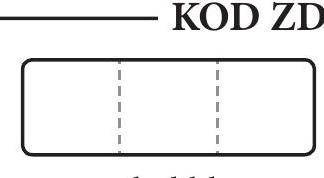
\includegraphics[max width=\textwidth, center]{2024_11_21_4c1aab2bfe739e583883g-01}\\
symbol klasy\\
KOD ZDAJĄCEGO\\
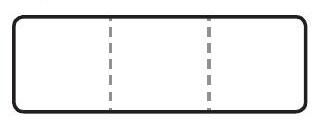
\includegraphics[max width=\textwidth, center]{2024_11_21_4c1aab2bfe739e583883g-01(1)}\\
symbol zdającego

\section*{Instrukcja dla zdającego}
\begin{enumerate}
  \item Sprawdź, czy arkusz egzaminacyjny zawiera 22 strony (zadania 1-33) i kartę odpowiedzi. Ewentualny brak stron zgłoś nauczycielowi nadzorującemu egzamin.
  \item Rozwiązania zadań i odpowiedzi zapisz w miejscu na to przeznaczonym.
  \item Pamiętaj, że pominięcie argumentacji lub istotnych obliczeń w rozwiązaniu zadań otwartych może spowodować, że za to rozwiązanie nie otrzymasz pełnej liczby punktów.
  \item Pisz czytelnie. Używaj długopisu/pióra tylko z czarnym tuszem/atramentem.
  \item Nie używaj korektora, a błędne zapisy wyraźnie przekreśl.
  \item Pamiętaj, że zapisy w brudnopisie nie będą oceniane.
  \item Podczas egzaminu możesz korzystać z zestawu wzorów matematycznych, cyrkla i linijki oraz kalkulatora prostego.
  \item Na tej stronie i na karcie odpowiedzi wpisz swój kod.
  \item Odpowiedzi do zadań zamkniętych przenieś na kartę odpowiedzi, zaznaczając je w części karty przeznaczonej dla zdającego.
  \item Nie wpisuj żadnych znaków w części przeznaczonej dla osoby sprawdzającej.
\end{enumerate}

\section*{Powodzenia!}
\section*{\(\square\) dysleksja}
STYCZEŃ 2019

Czas pracy:\\
170 minut

Liczba punktów\\
do uzyskania: 50

W zadaniach od 1. do 24. wybierz i zaznacz na karcie odpowiedzi poprawna odpowiedź.

Zadanie 1. (0-1)\\
Liczba przeciwna do liczby \((1-\sqrt{3})^{2}\) jest równa\\
A. \(4-2 \sqrt{3}\).\\
B. \(4+2 \sqrt{3}\).\\
C. \(-4-2 \sqrt{3}\).\\
D. \(-4+2 \sqrt{3}\).

Zadanie 2. (0-1)\\
Liczba odwrotna do liczby \(\frac{\left(5^{1,2}\right)^{3} \cdot \sqrt{5}^{0,8}}{5^{3}}\) jest równa\\
A. -5 .\\
B. 5 .\\
C. \(\frac{1}{5}\).\\
D. \(-\frac{1}{5}\).

\section*{Zadanie 3. (0-1)}
Wartość bezwzględna liczby \(3 \sqrt{2}-5\) jest równa\\
A. \(3 \sqrt{2}+5\).\\
B. \(5-3 \sqrt{2}\).\\
C. \(3 \sqrt{2}-5\).\\
D. \(-3 \sqrt{2}-5\).

\section*{Zadanie 4. (0-1)}
Kwotę 3000 zł ulokowano w banku na lokacie oprocentowanej 2\% w stosunku rocznym, przy czym odsetki są kapitalizowane co pół roku (nie uwzględniamy podatku od odsetek kapitałowych). Po trzech latach stan tej lokaty wyniesie\\
A. \(3000 \cdot\left(1+\frac{2}{100}\right)^{3} \mathrm{zt}\).\\
B. \(3000 \cdot\left(1+\frac{1}{100}\right)^{3} \mathrm{zt}\).\\
C. \(3000 \cdot\left(1+\frac{2}{100}\right)^{6} \mathrm{zt}\).\\
D. \(3000 \cdot\left(1+\frac{1}{100}\right)^{6} \mathrm{zt}\).

Zadanie 5. (0-1)\\
Zbiorem rozwiązań nierówności \((x+3)^{2} \leqslant 0\) jest\\
A. R.\\
B. \(\{-3\}\).\\
C. zbiór pusty.\\
D. \((-\infty,-3\rangle\).

Zadanie 6. (0-1)\\
Wyrażenie \((3 x-y)^{2}-(x-3 y)^{2}\) jest równe wyrażeniu\\
A. \(8 x^{2}-8 y^{2}\).\\
B. \(-12 x y+8 x^{2}-8 y^{2}\).\\
C. \(8 y^{2}-8 x^{2}\).\\
D. \(-12 x y+8 x^{2}+10 y^{2}\).\\

\includegraphics[max width=\textwidth, center]{2024_11_21_4c1aab2bfe739e583883g-03}

Zadanie 7. (0-1)\\
Układ równań liniowych \(\left\{\begin{aligned} 2 x-4 y & =3 \\ -3 x+6 y & =-4\end{aligned}\right.\)\\
A. nie ma rozwiązania.\\
B. ma dokładnie jedno rozwiązanie.\\
C. ma dokładnie dwa rozwiązania.\\
D. ma nieskończenie wiele rozwiązań.

\section*{Zadanie 8. (0-1)}
Iloczyn wszystkich pierwiastków równania \((2 x-3)\left(x^{2}+2 x\right)=0\) jest równy\\
A. \(-\frac{4}{3}\).\\
B. 0 .\\
C. 3.\\
D. -3 .

\section*{Zadanie 9. (0-1)}
W trójkącie prostokątnym jedna z przyprostokątnych ma długość 5, a przeciwprostokątna ma długość 13. Sinus większego kąta ostrego tego trójkąta jest równy\\
A. \(\frac{12}{13}\).\\
B. \(\frac{5}{13}\).\\
C. \(\frac{\sqrt{5}}{13}\).\\
D. \(\frac{5}{12}\).

Zadanie 10. (0-1)\\
Przyjmijmy, że \(\log 5=p\). Wtedy\\
A. \(p+1=\log \frac{1}{2}\).\\
B. \(2 p-2=\log \frac{1}{4}\).\\
C. \(p-1=\log \frac{1}{20}\).\\
D. \(p^{2}-2=\log \frac{1}{4}\).

\section*{Zadanie 11. (0-1)}
Wykres funkcji liniowej \(f(x)=-2 x+1\) przesunięto o trzy jednostki w prawo wzdłuż osi \(O X\). Otrzymano wykres funkcji\\
A. \(y=-2 x+7\).\\
B. \(y=-2 x+4\).\\
C. \(y=-2 x+5\).\\
D. \(y=-2 x-2\).

Zadanie 12. (0-1)\\
Funkcja liniowa \(f(x)=-3 x+2 b\) i funkcja liniowa \(g(x)=\frac{1}{2} x+2\) mają to samo miejsce zerowe. Wynika stąd, że\\
A. \(b=12\).\\
B. \(b=-12\).\\
C. \(b=6\).\\
D. \(b=-6\).\\

\includegraphics[max width=\textwidth, center]{2024_11_21_4c1aab2bfe739e583883g-05}

\section*{Zadanie 13. (0-1)}
Osią symetrii wykresu pewnej funkcji kwadratowej jest prosta o równaniu \(x=-3\), a wartość największa tej funkcji jest równa 4. Który ze wzorów może opisywać tę funkcję kwadratową?\\
A. \(y=2 \cdot(x+3)^{2}+4\)\\
B. \(y=-2 \cdot(x-3)^{2}+4\)\\
C. \(y=-2 \cdot(x+3)^{2}+4\)\\
D. \(y=-2 \cdot(x+3)^{2}-4\)

\section*{Zadanie 14. (0-1)}
Do wykresu funkcji wykładniczej \(y=a^{x}\) należy punkt \(A=\left(\frac{1}{3}, 2\right)\). Wynika stąd, że \(a\) jest równe\\
A. \(2^{-\frac{1}{3}}\).\\
B. \(\frac{1}{8}\).\\
C. 8 .\\
D. \(2^{\frac{1}{3}}\).

\section*{Zadanie 15. (0-1)}
Dany jest wykres funkcji \(y=f(x)\).\\
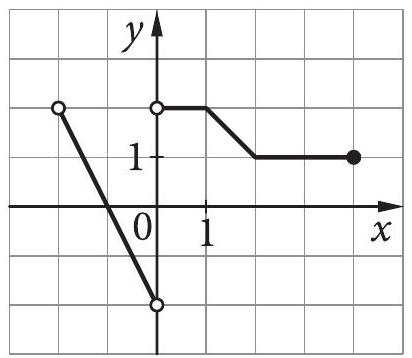
\includegraphics[max width=\textwidth, center]{2024_11_21_4c1aab2bfe739e583883g-06}

Zbiorem wartości funkcji \(f(x)\) jest przedział\\
A. \((-2,2\rangle\).\\
B. \((-2,2)\).\\
C. \(\langle-2,2\rangle\).\\
D. \(\langle-2,2)\).

\section*{Zadanie 16. (0-1)}
W niemonotonicznym ciągu geometrycznym dane są wyrazy \(a_{4}=16\) i \(a_{6}=1\). Piąty wyraz tego ciągu jest równy\\
A. -8 .\\
B. -4 .\\
C. 4.\\
D. 8 .

\section*{Zadanie 17. (0-1)}
Różnica \(r\) ciągu arytmetycznego o wzorze ogólnym \(a_{n}=5-3 n(n \geqslant 1)\) wynosi\\
A. 5 .\\
B. 3 .\\
C. 2 .\\
D. -3 .

\section*{Zadanie 18. (0-1)}
Dany jest okrąg o środku \(S=(4,-3)\) i promieniu \(r=5\). Liczba wszystkich punktów wspólnych tego okręgu z osiami układu współrzędnych jest równa\\
A. 1 .\\
B. 2 .\\
C. 3.\\
D. 4 .\\

\includegraphics[max width=\textwidth, center]{2024_11_21_4c1aab2bfe739e583883g-07}

Zadanie 19. (0-1)\\
Dana jest prosta o równaniu \(-2 x-4 y+3=0\). Wskaż równanie prostej, która jest do niej równoległa i przechodzi przez punkt \(P=(0,-2)\).\\
A. \(y=\frac{1}{2} x-2\)\\
B. \(y=-\frac{1}{2} x+2\)\\
C. \(y=2 x-2\)\\
D. \(y=-\frac{1}{2} x-2\)

\section*{Zadanie 20. (0-1)}
Dany jest romb, w którym kąt ostry ma miarę \(45^{\circ}\), a wysokość wynosi 6 cm . Ile wynosi pole tego rombu?\\
A. \(36 \sqrt{2} \mathrm{~cm}^{2}\)\\
B. \(36 \mathrm{~cm}^{2}\)\\
C. \(24 \sqrt{2} \mathrm{~cm}^{2}\)\\
D. \(18 \sqrt{2} \mathrm{~cm}^{2}\)

\section*{Zadanie 21. (0-1)}
Miara kąta środkowego w okręgu jest o \(40^{\circ}\) większa od miary kąta wpisanego opartego na tym samym łuku. Ile wynosi miara kąta wpisanego?\\
A. \(80^{\circ}\)\\
B. \(40^{\circ}\)\\
C. \(20^{\circ}\)\\
D. \(10^{\circ}\)

\section*{Zadanie 22. (0-1)}
Z połowy koła o promieniu 10 zbudowano powierzchnię boczną stożka. Ile wynosi promień podstawy tego stożka?\\
A. 10\\
B. 5\\
C. \(\sqrt{10}\)\\
D. \(\sqrt{5}\)

Zadanie 23. (0-1)\\
Jeśli graniastosłup ma 12 ścian, to liczba jego krawędzi jest równa\\
A. 20 .\\
B. 27 .\\
C. 30 .\\
D. 36 .

\section*{Zadanie 24. (0-1)}
W dwukrotnym rzucie sześcienną kostką do gry prawdopodobieństwo otrzymania sumy oczek równej 8 wynosi\\
A. \(\frac{1}{18}\).\\
B. \(\frac{1}{12}\).\\
C. \(\frac{1}{9}\).\\
D. \(\frac{5}{36}\).\\

\includegraphics[max width=\textwidth, center]{2024_11_21_4c1aab2bfe739e583883g-09}

Zadanie 25. (0-2)\\
Rozwiąż nierówność \((2 x-3)^{2}-4 \geqslant 0\).\\

\includegraphics[max width=\textwidth, center]{2024_11_21_4c1aab2bfe739e583883g-10}

Odpowiedź:

Zadanie 26. (0-2)\\
Dla kąta ostrego \(\alpha\) dany jest \(\cos \alpha=\frac{2}{3}\). Oblicz wartość wyrażenia \(\sqrt{\operatorname{tg}^{2} \alpha+1}\).

Więcej arkuszy znajdziesz na stronie: \href{http://arkusze.pl}{arkusze.pl}\\

\includegraphics[max width=\textwidth, center]{2024_11_21_4c1aab2bfe739e583883g-11}

Odpowiedź:

\begin{center}
\begin{tabular}{|l|l|c|c|}
\hline
\multirow{2}{*}{\begin{tabular}{c}
Wypełnia \\
sprawdzający \\
\end{tabular}} & Nr zadania & 25 & 26 \\
\cline { 2 - 4 }
 & Maks. liczba pkt & 2 & 2 \\
\cline { 2 - 4 }
 & Uzyskana liczba pkt &  &  \\
\hline
\end{tabular}
\end{center}

\section*{Zadanie 27. (0-2)}
Ze zbioru liczb naturalnych dwucyfrowych mniejszych od 30 losujemy dwa razy po jednej liczbie bez zwracania. Oblicz prawdopodobieństwo zdarzenia \(A\), w którym obie wylosowane liczby będą podzielne przez 3.

Więcej arkuszy znajdziesz na stronie: \href{http://arkusze.pl}{arkusze.pl}\\

\includegraphics[max width=\textwidth, center]{2024_11_21_4c1aab2bfe739e583883g-12}

Odpowiedź:

Zadanie 28. (0-2)\\
W ciągu arytmetycznym \(\left(a_{n}\right)\) określonym dla \(n \geqslant 1\), dane są wyrazy \(a_{2}=-2\) i \(a_{5}=7\). Oblicz sumę wyrazów tego ciągu, od wyrazu piątego do wyrazu dwudziestego.

Więcej arkuszy znajdziesz na stronie: \href{http://arkusze.pl}{arkusze.pl}\\

\includegraphics[max width=\textwidth, center]{2024_11_21_4c1aab2bfe739e583883g-13}

Odpowiedź:

\begin{center}
\begin{tabular}{|l|l|c|c|}
\hline
\multirow{2}{*}{\begin{tabular}{c}
Wypełnia \\
sprawdzający \\
\end{tabular}} & Nr zadania & 27 & 28 \\
\cline { 2 - 4 }
 & Maks. liczba pkt & 2 & 2 \\
\cline { 2 - 4 }
 & Uzyskana liczba pkt &  &  \\
\hline
\end{tabular}
\end{center}

Zadanie 29. (0-2)\\
Udowodnij, że dla dowolnej liczby rzeczywistej ujemnej prawdziwa jest nierówność

\[
9 x+\frac{1}{x} \leqslant-6 .
\]

Więcej arkuszy znajdziesz na stronie: \href{http://arkusze.pl}{arkusze.pl}\\

\includegraphics[max width=\textwidth, center]{2024_11_21_4c1aab2bfe739e583883g-14}

\section*{Zadanie 30. (0-3)}
W kwadracie \(A B C D\), w którym punkt \(E\) jest środkiem boku \(C D\), poprowadzono przekątną \(B D\) i odcinek \(A E\), które przecięły się w punkcie \(P\). Uzasadnij, że suma pól trójkątów \(A B P\) i \(D E P\) stanowi \(\frac{5}{12}\) pola kwadratu \(A B C D\).\\
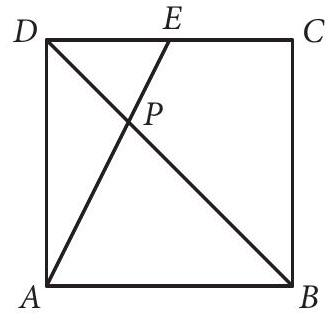
\includegraphics[max width=\textwidth, center]{2024_11_21_4c1aab2bfe739e583883g-15(1)}

Więcej arkuszy znajdziesz na stronie: \href{http://arkusze.pl}{arkusze.pl}

\begin{center}
\begin{tabular}{|c|c|c|c|c|c|c|c|c|c|c|c|c|c|c|c|c|c|c|c|c|c|c|c|c|c|c|c|c|c|}
\hline
 &  &  &  &  &  &  &  &  &  &  &  &  &  &  &  &  &  &  &  &  &  &  &  &  &  &  &  &  &  \\
\hline
 &  &  &  &  &  &  &  &  &  &  &  &  &  &  &  &  &  &  &  &  &  &  &  &  &  &  &  &  &  \\
\hline
 &  &  &  &  &  &  &  &  &  &  &  &  &  &  &  &  &  &  &  &  &  &  &  &  &  &  &  &  &  \\
\hline
 &  &  &  &  &  &  &  &  &  &  &  &  &  &  &  &  &  &  &  &  &  &  &  &  &  &  &  &  &  \\
\hline
 &  &  &  &  &  &  &  &  &  &  &  &  &  &  &  &  &  &  &  &  &  &  &  &  &  &  &  &  &  \\
\hline
 &  &  &  &  &  &  &  &  &  &  &  &  &  &  &  &  &  &  &  &  &  &  &  &  &  &  &  &  &  \\
\hline
 &  &  &  &  &  &  &  &  &  &  &  &  &  &  &  &  &  &  &  &  &  &  &  &  &  &  &  &  &  \\
\hline
 &  &  &  &  &  &  &  &  &  &  &  &  &  &  &  &  &  &  &  &  &  &  &  &  &  &  &  &  &  \\
\hline
 &  &  &  &  &  &  &  &  &  &  &  &  &  &  &  &  &  &  &  &  &  &  &  &  &  &  &  &  &  \\
\hline
 &  &  &  &  &  &  &  &  &  &  &  &  &  &  &  &  &  &  &  &  &  &  &  &  &  &  &  &  &  \\
\hline
 &  &  &  &  &  &  &  &  &  &  &  &  &  &  &  &  &  &  &  &  &  &  &  &  &  &  &  &  &  \\
\hline
 &  &  &  &  &  &  &  &  &  &  &  &  &  &  &  &  &  &  &  &  &  &  &  &  &  &  &  &  &  \\
\hline
 &  &  &  &  &  &  &  &  &  &  &  &  &  &  &  &  &  &  &  &  &  &  &  &  &  &  &  &  &  \\
\hline
 &  &  &  &  &  &  &  &  &  &  &  &  &  &  &  &  &  &  &  &  &  &  &  &  &  &  &  &  &  \\
\hline
 &  &  &  &  &  &  &  &  &  &  &  &  &  &  &  &  &  &  &  &  &  &  &  &  &  &  &  &  &  \\
\hline
 &  &  &  &  &  &  &  &  &  &  &  &  &  &  &  &  &  &  &  &  &  &  &  &  &  &  &  &  &  \\
\hline
 &  &  &  &  &  &  &  &  &  &  &  &  &  &  &  &  &  &  &  &  &  &  &  &  &  &  &  &  &  \\
\hline
 &  &  &  &  &  &  &  &  &  &  &  &  &  &  &  &  &  &  &  &  &  &  &  &  &  &  &  &  &  \\
\hline

\includegraphics[max width=\textwidth]{2024_11_21_4c1aab2bfe739e583883g-15}
 &  &  &  &  &  &  &  &  &  &  &  &  &  &  &  &  &  &  &  &  &  &  &  &  &  &  &  &  &  \\
\hline
 &  &  &  &  &  &  &  &  &  &  &  &  &  &  &  &  &  &  &  &  &  &  &  &  &  &  &  &  &  \\
\hline
 &  &  &  &  &  &  &  &  &  &  &  &  &  &  &  &  &  &  &  &  &  &  &  &  &  &  &  &  &  \\
\hline
 &  &  &  &  &  &  &  &  &  &  &  &  &  &  &  &  &  &  &  &  &  &  &  &  &  &  &  &  &  \\
\hline
 &  &  &  &  &  &  &  &  &  &  &  &  &  &  &  &  &  &  &  &  &  &  &  &  &  &  &  &  &  \\
\hline
 &  &  &  &  &  &  &  &  &  &  &  &  &  &  &  &  &  &  &  &  &  &  &  &  &  &  &  &  &  \\
\hline
 &  &  &  &  &  &  &  &  &  &  & \textbackslash  & \textbackslash  &  &  &  &  &  &  &  &  &  &  &  &  &  &  &  &  &  \\
\hline
 &  &  &  &  &  &  &  &  &  &  &  &  &  &  &  &  &  &  &  &  &  &  &  &  &  &  &  &  &  \\
\hline
 &  &  &  &  &  &  &  &  &  &  &  &  &  &  &  &  &  &  &  &  &  &  &  &  &  &  &  &  &  \\
\hline
 &  &  &  &  &  &  &  &  &  &  &  &  &  &  &  &  &  &  &  &  &  &  &  &  &  &  &  &  &  \\
\hline
 &  &  &  &  &  &  &  &  &  &  &  &  &  &  &  &  &  &  &  &  &  &  &  &  &  &  &  &  &  \\
\hline
 &  &  &  &  &  &  &  &  &  &  &  &  &  &  &  &  &  &  &  &  &  &  &  &  &  &  &  &  &  \\
\hline
 &  &  &  &  &  &  &  &  &  &  &  &  &  &  &  &  &  &  &  &  &  &  &  &  &  &  &  &  &  \\
\hline
\end{tabular}
\end{center}

\begin{center}
\begin{tabular}{|c|l|c|c|}
\hline
\multirow{3}{*}{\begin{tabular}{c}
Wypełnia \\
sprawdzający \\
\end{tabular}} & Nr zadania & 29 & 30 \\
\cline { 2 - 4 }
 & Maks. liczba pkt & 2 & 3 \\
\cline { 2 - 4 }
 & Uzyskana liczba pkt &  &  \\
\hline
\end{tabular}
\end{center}

Zadanie 31. (0-4)\\
Wyznacz wzór funkcji kwadratowej w postaci ogólnej, jeżeli wierzchołek paraboli, która jest jej wykresem, znajduje się w punkcie \(W=(-1,5)\), a ta funkcja w przedziale \(\langle-2,2\rangle\) osiąga najmniejszą wartość równą -4 .

Więcej arkuszy znajdziesz na stronie: \href{http://arkusze.pl}{arkusze.pl}\\

\includegraphics[max width=\textwidth, center]{2024_11_21_4c1aab2bfe739e583883g-16}\\
Więcej arkuszy znajdziesz na stronie: \href{http://arkusze.pl}{arkusze.pl}\\

\includegraphics[max width=\textwidth, center]{2024_11_21_4c1aab2bfe739e583883g-17}

Odpowiedź:

\begin{center}
\begin{tabular}{|l|l|c|}
\hline
\multirow{2}{*}{\begin{tabular}{c}
Wypełnia \\
sprawdzający \\
\end{tabular}} & Nr zadania & 31 \\
\cline { 2 - 3 }
 & Maks. liczba pkt & 4 \\
\cline { 2 - 3 }
 & Uzyskana liczba pkt &  \\
\hline
\end{tabular}
\end{center}

Zadanie 32. (0-5)\\
W trójkącie równoramiennym \(A B C\) dane są wierzchołki podstawy \(A=(2,1)\) i \(B=(6,5)\) oraz\\
wysokość \(|C D|=\frac{7 \sqrt{2}}{2}\). Oblicz współrzędne wierzchołka \(C\), jeżeli wiadomo, że obie te współrzędne są dodatnie.

Więcej arkuszy znajdziesz na stronie: \href{http://arkusze.pl}{arkusze.pl}\\

\includegraphics[max width=\textwidth, center]{2024_11_21_4c1aab2bfe739e583883g-18}\\
Więcej arkuszy znajdziesz na stronie: \href{http://arkusze.pl}{arkusze.pl}\\

\includegraphics[max width=\textwidth, center]{2024_11_21_4c1aab2bfe739e583883g-19}

Odpowiedź:

\begin{center}
\begin{tabular}{|l|l|c|}
\hline
\multirow{2}{*}{\begin{tabular}{c}
Wypelnia \\
sprawdzający \\
\end{tabular}} & Nr zadania & 32 \\
\cline { 2 - 3 }
 & Maks. liczba pkt & 5 \\
\cline { 2 - 3 }
 & Uzyskana liczba pkt &  \\
\hline
\end{tabular}
\end{center}

Zadanie 33. (0-4)\\
W ostrosłupie czworokątnym prawidłowym pole jednej ściany bocznej wynosi 12, a cosinus kąta nachylenia ściany bocznej do płaszczyzny podstawy jest równy \(\frac{1}{3}\). Oblicz objętość tego ostrosłupa.\\

\includegraphics[max width=\textwidth, center]{2024_11_21_4c1aab2bfe739e583883g-20}\\
Więcej arkuszy znajdziesz na stronie: \href{http://arkusze.pl}{arkusze.pl}\\

\includegraphics[max width=\textwidth, center]{2024_11_21_4c1aab2bfe739e583883g-21}

Odpowiedź:

\begin{center}
\begin{tabular}{|l|l|c|}
\hline
\multirow{2}{*}{\begin{tabular}{c}
Wypelnia \\
sprawdzający \\
\end{tabular}} & Nr zadania & 33 \\
\cline { 2 - 3 }
 & Maks. liczba pkt & 4 \\
\cline { 2 - 3 }
 & Uzyskana liczba pkt &  \\
\hline
\end{tabular}
\end{center}


\includegraphics[max width=\textwidth, center]{2024_11_21_4c1aab2bfe739e583883g-22}\\
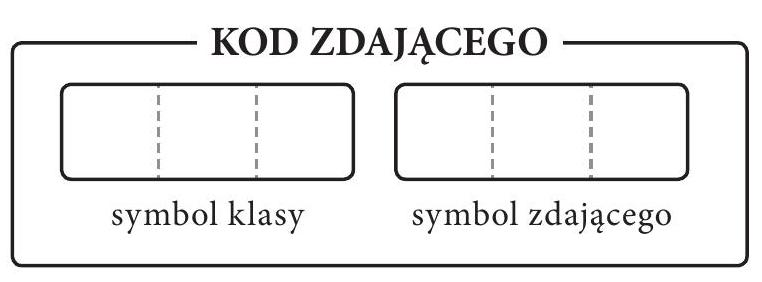
\includegraphics[max width=\textwidth, center]{2024_11_21_4c1aab2bfe739e583883g-23}

KARTA ODPOWIEDZI

\begin{center}
\begin{tabular}{|c|c|c|c|c|c|}
\hline
 & \begin{tabular}{l}
Nr \\
zad. \\
\end{tabular} & \multicolumn{4}{|c|}{Odpowiedzi} \\
\hline
 & 1 & A & B & C & D \\
\hline
 & 2 & A & B & C & D \\
\hline
 & 3 & A & B & C & D \\
\hline
₪ٌ & 4 & A & B & C & D \\
\hline
气㐅\_ & 5 & A & B & C & D \\
\hline

\includegraphics[max width=\textwidth]{2024_11_21_4c1aab2bfe739e583883g-23(1)}
 & 6 & A & B & C & D \\
\hline
\( \left.{ }^{\prime}\right]_{0} \) & 7 & A & B & C & C \\
\hline
鿌 & 8 & A & B & C & D \\
\hline
N & 9 & A & B & C & D \\
\hline
- & 10 & A & B & C & D \\
\hline
‘ত্ট & 11 & A & B & C & D \\
\hline
凡 & 12 & A & B & C & D \\
\hline
和 & 13 & A & B & C & D \\
\hline
ঠ & 14 & A & B & C & D \\
\hline
هِ & 15 & A & B & C & D \\
\hline
 & 16 & A & B & C & D \\
\hline
 & 17 & A & B & C & D \\
\hline
 & 18 & A & B & C & D \\
\hline
 & 19 & A & B & C & D \\
\hline
 & 20 & A & B & C & D \\
\hline
 & 21 & A & B & C & D \\
\hline
 & 22 & A & B & C & D \\
\hline
 & 23 & A & B & C & D \\
\hline
 & 24 & A & B & C & D \\
\hline
\end{tabular}
\end{center}

WYPEENIA SPRAWDZAJĄCY

\begin{center}
\begin{tabular}{|c|c|c|c|c|c|c|}
\hline
\multirow{2}{*}{\begin{tabular}{c}
Nr \\
zad. \\
\end{tabular}} & \multicolumn{6}{|c|}{Punkty} \\
\hline
 & \(\mathbf{0}\) & \(\mathbf{1}\) & \(\mathbf{2}\) & \(\mathbf{3}\) & \(\mathbf{4}\) & \(\mathbf{5}\) \\
\hline
\(\mathbf{2 5}\) & \(\square\) & \(\square\) & \(\square\) &  &  &  \\
\hline
\(\mathbf{2 6}\) & \(\square\) & \(\square\) & \(\square\) &  &  &  \\
\hline
\(\mathbf{2 7}\) & \(\square\) & \(\square\) & \(\square\) &  &  &  \\
\hline
\(\mathbf{2 8}\) & \(\square\) & \(\square\) & \(\square\) &  &  &  \\
\hline
\(\mathbf{2 9}\) & \(\square\) & \(\square\) & \(\square\) &  &  &  \\
\hline
\(\mathbf{3 0}\) & \(\square\) & \(\square\) & \(\square\) & \(\square\) &  &  \\
\hline
\(\mathbf{3 1}\) & \(\square\) & \(\square\) & \(\square\) & \(\square\) & \(\square\) &  \\
\hline
\(\mathbf{3 2}\) & \(\square\) & \(\square\) & \(\square\) & \(\square\) & \(\square\) & \(\square\) \\
\hline
\(\mathbf{3 3}\) & \(\square\) & \(\square\) & \(\square\) & \(\square\) & \(\square\) &  \\
\hline
\end{tabular}
\end{center}


\end{document}